\section{编译C程序的工作原理}
\begin{frame}\ft{\secname}
  C是一种高级语言,它需要编译器将其转换为可执行代码,以使得程序能在机器上运行。 

  以下介绍在MAC或Linux上使用gcc编译器的几个步骤。

\end{frame}


\begin{frame}[fragile]\ft{\secname}
  \begin{itemize}

  \item[(1)] 首先使用编辑器(如vi或emacs等)创建一个C程序,并将其保存为hello.c。

    \begin{lstlisting}
$ emacs hello.c
    \end{lstlisting}
  \end{itemize}
\end{frame}

\begin{frame}[fragile]\ft{\secname}
  \begin{itemize}
  \item[] 
    在编辑界面输入以下内容:
    \lstinputlisting[]{ch01/code/hello.c}

  \end{itemize}
\end{frame}

\begin{frame}[fragile]\ft{\secname}
  \begin{itemize}
  \item[(2)] 然后用以下命令编译,并查看当前目录下的文件。
    \begin{lstlisting}[backgroundcolor=\color{red!10}]
$ gcc -Wall hello.c –o hello
$ ls
  hello    hello.c
\end{lstlisting}

\begin{itemize}
\item 选项 \blue{\lstinline|-Wall|} 启动所有编译器的警告信息。建议使用该选项以生成更好的代码。
\item 选项 \blue{\lstinline|-o|} 用来制定输出文件名。如果缺省该选项,则输出文件将默认为 \blue{\lstinline|a.out|}。
\end{itemize}
    
  \end{itemize}
\end{frame}

\begin{frame}[fragile]\ft{\secname}
  \begin{itemize}
  \item[(3)] 编译通过后,将会生成可执行文件。可用以下命令来运行:
    \begin{lstlisting}[backgroundcolor=\color{red!10}]
$ ./hello
Hello World!
    \end{lstlisting}
  \end{itemize}
\end{frame}



\begin{frame}[fragile]\ft{\secname}
  \href{https://blog.csdn.net/elfprincexu/article/details/45043971}{编译器将一个C程序转换为一个可执行文件},需经历了4个阶段:
  \begin{itemize}
  \item 预处理
  \item 编译
  \item 汇编
  \item 链接
  \end{itemize}

  \begin{figure}
    \centering
    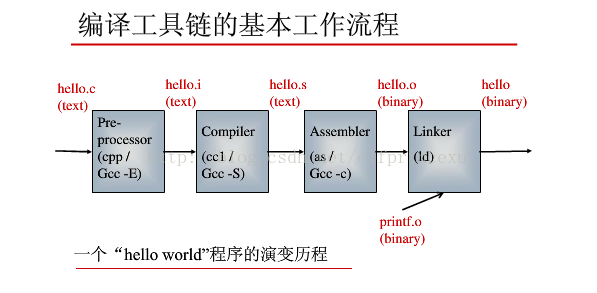
\includegraphics[width=4in]{ch01/images/compile.png}
    \caption{编译过程}
    \label{fig:1}
  \end{figure}
  
\end{frame}


\begin{frame}[fragile]\ft{\secname}
  执行以下命令,会在当前目录下生成所有的中间文件以及可执行文件。
  \begin{lstlisting}[backgroundcolor=\color{red!10}]
    $ gcc -Wall -save-temps hello.c –o hello 
    $ ls 
    hello     hello.c   hello.o
    hello.i   hello.s
  \end{lstlisting}
\end{frame}


\begin{frame}[fragile]\ft{\secname} 
  \begin{itemize}
  \item[(1)] \red{预处理阶段}
\begin{lstlisting}[backgroundcolor=\color{red!10}]
$ gcc -E hello.c –o hello.i 
\end{lstlisting}    
\end{itemize}

在该阶段,
    \begin{itemize}
    \item 去掉注释
    \item 宏的展开
    \item 头文件的展开
    \item 选项 \blue{\lstinline|-E|} 的作用是让gcc在预处理结束后停止编译过程。
    \end{itemize}   
\end{frame}


\begin{frame}[fragile]\ft{\secname}
  \begin{lstlisting}[basicstyle=\ttfamily\footnotesize,backgroundcolor=\color{red!10}]
    $ less hello.i
    $ ls 
    ...
    extern int printf (const char *__restrict __format, ...);
    ...
    # 868 "/usr/include/stdio.h" 3 4
    # 5 "hello.c" 2
    # 5 "hello.c"

    int main(void)
    {
      printf("Hello World!\n");
      return 0;
    }
  \end{lstlisting}
\end{frame}


% \begin{frame}[fragile]\ft{\secname}
%   \blue{分析:}在以上内容中,源文件被附加了很多信息,但在末尾代码仍被保留。{\ttfamily printf()}函数中包含了{\ttfamily a+b}而非{\ttfamily add(a,b)},因为宏已被展开。注释被去除掉。{\ttfamily\#include<stdio.h>}没有了,取而代之的是很多代码。因此,头文件已被展开,并且被包含到了源文件中。

% \end{frame}


\begin{frame}[fragile]\ft{\secname}
  \begin{itemize}
  \item[(2)] 编译阶段
\begin{lstlisting}[backgroundcolor=\color{red!10}]
$ gcc -S hello.i –o hello.s
\end{lstlisting}
\end{itemize}

在该阶段,
\begin{itemize}
\item 检查代码的规范性、是否有语法错误等
\item 检查无误后,将代码翻译成汇编语言
\item 选项 \blue{\lstinline|-S|} 只进行编译,不进行汇编,生成汇编代码。 
\end{itemize}

\end{frame}


\begin{frame}[fragile]\ft{\secname}
  \begin{lstlisting}[basicstyle=\ttfamily\footnotesize,backgroundcolor=\color{red!10}]
    $ less hello.s
    ...
    movl    $0, -4(%rbp)
    movl    $5, -8(%rbp)
    movl    $4, -12(%rbp)
    movl    -8(%rbp), %eax
    addl    -12(%rbp), %eax
    movl    %eax, %esi
    movb    $0, %al
    callq   _printf
    xorl    %esi, %esi
    ...      
  \end{lstlisting}
  % 以上内容表明这是汇编语言,能为汇编器所识别。
\end{frame}


\begin{frame}[fragile]\ft{\secname}
  \begin{itemize}
  \item[(3 )] 汇编阶段
\begin{lstlisting}[backgroundcolor=\color{red!10}]
$ gcc -c hello.s –o hello.o
\end{lstlisting}   
\end{itemize}

在该阶段,
\begin{itemize}
\item 将通过汇编器将 \lstinline|hello.s| 转换成  二进制机器指令文件\lstinline|hello.o|。
\item 只会将现有代码转换成机器语言,而诸如 \lstinline|printf()| 的函数调用则不会。
\item 选项 \blue{\lstinline|-c|} 的作用是将汇编代码转换为二进制目标代码。
\end{itemize}
\end{frame}


\begin{frame}[fragile]\ft{\secname}
  \begin{lstlisting}[backgroundcolor=\color{red!10}]
    $ less hello.o
    <CF><FA><ED><FE>^G^@^@^A^C^@^@^@^A^@^@^@^D^@^@^@^@^B^@^@^@ ^@^@^@^@^@^@^Y^@^@^@<88>^A^@^@^@^@^@^@^@^
    ...      
  \end{lstlisting}

\end{frame}


\begin{frame}[fragile]\ft{\secname}
  \begin{itemize}
  \item[(4)] 链接阶段
  \item[] 
    这是最后一个阶段,将完成所有函数调用及其定义的链接工作。链接器知道所有这些函数在何处执行。链接器也会做一些额外的工作,以添加一些启动和结束程序所需的额外代码。 
  \end{itemize}
\end{frame}


\begin{frame}[fragile]\ft{\secname}
  在命令行中输入以下命令,可看出从目标文件到可执行文件时文件大小的变化。这是因为链接器为我们的程序添加了额外的代码。
  \begin{lstlisting}[basicstyle=\ttfamily\footnotesize,backgroundcolor=\color{red!10}]
    $ size hello.o
    __TEXT  __DATA  __OBJC  others    dec         hex
    145     0       0       32      177         b1        
    $ size hello
    __TEXT  __DATA  __OBJC  others    dec         hex
    4096      4096    0  4294971392 4294979584 100003000
  \end{lstlisting}

\end{frame}
